% use "amsart" instead of "article" for AMSLaTeX format
\documentclass[a4paper,11.5pt]{report}   
\renewcommand{\baselinestretch}{1.5} 

\usepackage[strings]{underscore}
\usepackage{datetime}

\newdateformat{monthyeardate}{%
  \monthname[\THEMONTH], \THEYEAR}

\usepackage{enumerate}

\usepackage{setspace}

%\usepackage[margin=1.2in]{geometry}

\usepackage[a4paper,bindingoffset=0.4in,%
            left=1in,right=1in,top=1in,bottom=1in,%
            footskip=.25in]{geometry}
            


% ... or a4paper or a5paper or
\geometry{a4paper}      
             		
% Activate to begin paragraphs with an empty line rather than an indent
\usepackage[parfill]{parskip}   

 % Use pdf, png, jpg, or eps§ with pdflatex; use eps in DVI mode		
\usepackage{graphicx, wrapfig}				

\setcounter{secnumdepth}{4}

\usepackage{nomencl}
\makenomenclature

\usepackage{lipsum}

\usepackage{gensymb}

%\usepackage[monochrome]{color}
%\usepackage[utf8]{inputenc}


\usepackage{float}

\usepackage{amsmath}
	\numberwithin{figure}{section}
	\numberwithin{table}{section}
	\numberwithin{equation}{section}

\usepackage{amsmath}
	\numberwithin{equation}{section}
	\newcommand*{\Scale}[2][4]{\scalebox{#1}{$#2$}}%
	
\usepackage{multirow}

\usepackage{appendix}

\usepackage{array}

%\newcolumntype{P}[1]{>{\centering\arraybackslash}p{#1}}

\usepackage{blindtext}

\usepackage[export]{adjustbox}[2011/08/13]
	
\usepackage{gensymb}
	
\usepackage{colortbl}

\usepackage{longtable}

\usepackage{tabularx}

\usepackage{enumerate}

\newcommand{\gray}{\rowcolor[gray]{.90}}

\makeatletter
\newcommand*{\rom}[1]{\expandafter\@slowromancap\romannumeral #1@}
\makeatother

\usepackage{rotating}

\bibliographystyle{unsrtnat} 
\usepackage[sort&compress,numbers]{natbib}


\usepackage[final]{pdfpages}

\usepackage{caption}

\usepackage[% line break after label
   singlelinecheck=off, font=bf]{caption}
%\newcommand{\rom}[1]{%
%  \textup{\expandafter{\romannumeral#1}}%
%}

\usepackage{tocloft}
\renewcommand{\cftpartleader}{\cftdotfill{\cftdotsep}} % for parts
\renewcommand{\cftchapleader}{\cftdotfill{\cftdotsep}} % for chapters
 \renewcommand\cftchapafterpnum{\vskip10pt}

 
%\usepackage{titletoc}% http://ctan.org/pkg/titletoc
%\titlecontents*{chapter}% <section-type>
%  [0pt]% <left>
%  {}% <above-code>
%  {\bfseries\chaptername\ \thecontentslabel.\quad}% <numbered-entry-format>
%  {}% <numberless-entry-format>
%  {\bfseries\hfill\contentspage}% <filler-page-format>


\usepackage{subfig}					%use figure packagesx

\makeatletter

\newcommand\frontmatter{%
    \cleardoublepage
  %\@mainmatterfalse
  \pagenumbering{Roman}}

\newcommand\mainmatter{%
    \cleardoublepage
 % \@mainmattertrue
  \pagenumbering{arabic}}

\newcommand\backmatter{%
  \if@openright
    \cleardoublepage
  \else
    \clearpage
  \fi
 % \@mainmatterfalse
   }

\makeatother

\usepackage{fancyhdr}
\fancyhf{}
  \fancyhf[lef,rof]{\thepage}%
\pagestyle{fancy}
\fancypagestyle{plain}{%
  \fancyhf{}%
  \renewcommand{\headrulewidth}{0pt}%
  \fancyhf[rof]{\thepage}%
}

\usepackage{memhfixc}

\renewcommand{\contentsname}{Table of Contents}

\usepackage{pdflscape}

\usepackage{lscape}

\usepackage{textcomp}

%\usepackage[libertine,cmintegrals,cmbraces,vvarbb]{newtxmath}

%\usepackage[sorting=none]{biblatex}

\usepackage{notoccite}

\usepackage{titlesec}
\usepackage{appendix, apptools}
\AtAppendix{%
\titleformat{\chapter}[display]{\vspace*{-30pt}\bfseries\huge}{\chaptername~\thechapter}{1em}{}
\titlespacing*{\chapter}{0pt}{0pt}{0pt}}%

\makeatletter
\newcommand{\mypm}{\mathbin{\mathpalette\@mypm\relax}}
\newcommand{\@mypm}[2]{\ooalign{%
  \raisebox{.1\height}{$#1+$}\cr
  \smash{\raisebox{-.6\height}{$#1-$}}\cr}}
\makeatother

\usepackage{afterpage}
\newcommand\blankpage{%
    \null
    \thispagestyle{empty}%
    \addtocounter{page}{-1}%
    \newpage}
    



%\title{
%Development an Educational Game to Teach SQL Programming
%}
%\author{
%Amarnath Kakkar \\
%\normalsize University of Bath
%}
%\date{}							% Activate to display a given date or no date


\begin{document}

\frontmatter


%titlepage
\clearpage\thispagestyle{empty}
\begin{center}
\begin{minipage}{0.9\linewidth}
    \centering
%University logo
    \vspace{0.8cm}
    
\includegraphics[width=0.4\linewidth]{logobath.jpg}\par
    
    \vspace{2.5cm}
%Thesis title
    \vspace{0.2cm}
    {\uppercase{\Large \textbf{Development of an Educational Game to Teach Iteration and Conditional Statements} \par}}
    \vspace{3cm}
%Author's name
    {\Large \textbf{Amarnath Kakkar}\par}
        \vspace{3cm}
% $^{\circ}$
    {\large A final year project submitted in partial fulfilment for the degree of Bachelor's in Computer Science and Mathematics with Honours\par}
    {\large University of Bath\par}
    \vspace{4.5cm}
%supervisor and date
    {\large \textbf{\monthyeardate\today}\par}
    \vspace{1cm}
\end{minipage}
\end{center}

\afterpage{\blankpage}




\clearpage\thispagestyle{empty}
\begin{center}
\begin{minipage}{0.9\linewidth}
%University logo

\vspace{10cm}
{This dissertation may be made available for consultation within the University Library and may be photocopied or lent to other libraries for the purposes of consultation.\par}
\vspace{1cm}
Signed: 
   	
	
\end{minipage}
\end{center}

\newpage



    
\clearpage\thispagestyle{empty}
\begin{center}
\begin{minipage}{1\linewidth}
%Thesis title
%    \vspace{0.2cm}
%    {\uppercase{\large {Submitted in partial fulfilment for the degree of masters in aerospace engineering} \par}}
    \vspace{2cm}
%%Author's name
    {\LARGE Development of an Educational Game to Teach Iteration and Conditional Statements \par}
    \vspace{1cm}	
    {\large Submitted by: Amarnath Kakkar\par}
	
    \vspace{1.5cm}
    {\Large \textbf{COPYRIGHT}\par}
    \vspace{0.5cm}
    {Attention is drawn to the fact that copyright of this dissertation rests with its author. The Intellectual Property Rights of the products produced as part of the project belong to the author unless otherwise specified below, in accordance with the University of Bath?s policy on intellectual property
(see http://www.bath.ac.uk/ordinances/22.pdf).
This copy of the dissertation has been supplied on condition that anyone who consults it is understood to recognise that its copyright rests with its author and that no quotation from the dissertation and no information derived from it may be published without the prior written consent of the author.\par}

     \vspace{0.5cm}
     {\Large \textbf{Declaration}\par}
      \vspace{0.5cm}
      {This dissertation is submitted to the University of Bath in accordance with the requirements of the degree of Bachelor of Science in the Department of Computer Science. No portion of the work in this dissertation has been submitted in sup- port of an application for any other degree or qualification of this or any other university or institution of learning. Except where specifically acknowledged, it is the work of the author.\par}
    
     \vspace{2.5cm}
%% $^{\circ}$
    {\large Department of Computer Science\par}
    {\large University of Bath\par}
    \vspace{0.5cm}
%supervisor and date
    {\large Supervisor: Dr. Alan Hayes}\par
    {\large \textbf{\monthyeardate\today}\par}
    \vspace{1cm}
\end{minipage}
\end{center}

\newpage

\hfill

\section*{\Huge{Abstract}}

To be written.



\newpage

\addtocontents{toc}{\protect\setstretch{1}}
\tableofcontents

\newpage
{%
\let\oldnumberline\numberline%
\renewcommand{\numberline}{\figurename~\oldnumberline}%
\listoffigures%
}

\newpage
\listoftables  

\newpage
\hfill

\section*{\Huge{Outline of Project}}

To be written.

\newpage
\hfill
\section*{\Huge{Acknowldgements}}

To be written.
 
\afterpage{\blankpage}

\mainmatter

\chapter{Introduction}
\afterpage{\blankpage}

\chapter{Literature and Technology Survey}
%\section{Aims of This Section}

%This Literature Review aims to bring together various studies, and provide an insight into the use of games for educational purposes. It also aims to critically evaluate the material for any consistencies or inconsistencies, and to hopefully provide another perspective on the field.

%\subsection{Defining Serious Games}
%In the area of gamification, various definitions of serious games are found. Most commonly, and perhaps quite broadly, the term 'serious game', is defined as, digital games used for purposes other than mere entertainment \cite{Susi2416}.  While a variety of definitions have been suggested, this dissertation will use the definition suggested by \cite{Garris2002} who saw it as "instructional games that are designed for training or to promote learning" together with "games that do not have entertainment, enjoyment or fun as their primary purpose"  \cite{MichaelChen2006}. However, it is not to say that serious games should not be entertaining, enjoyable or fun.

%\subsection{Outline of Review}
%This review will; identify the benefits of serious games, and make clear any negatives, go through examples of serious games and their approaches, including any specific game design elements implemented, and outline any techniques that seem to be of positive influence or negative influence, look into existing resources for teaching SQL and outline the trade-offs with each approach, finally bring together these ideas summarise various points.

%\section{Benefits of Serious Games}
%Today's students are brought up in the digital era. \cite{Prensky2001} refers to them as 'Digital Natives', that have experienced a new form of video game play, which brings opportunities with great potential for their learning. Thus potentially making games great learning environments within education. However, \cite{Girard2013} summarises that there is need for more empirical research to determine the effectiveness of serious games. On the other hand, \cite{Pieter2013} reports that in general, serious games are more effective than traditional teaching methods, and that more studies are required to determine the effects of various features.

%In this section, we will outline some of the empirical researches that exist on the internet.

%\subsection{}

%\section{Examples of Serious Games}
%\subsection{Game Design Elements}
%\section{Existing Methods for Teaching SQL}
%\section{Summary}

\section{Video Games}

%The academic study of games, ludology, is a relatively new and emerging field. As the video game revolution took off in the late 20th century, so did academic interest in games. 

%Video games for entertainment have dominated the market, 

%The academic study of games, is a relatively new and emerging field. Games are naturally creative things, however academics see the potential in games for a variety of different reasons, and so game design frameworks have been developed to help design and create games.

The video games industry is growing very rapidly. The value of the video games market was predicted at \$122 billion USD in 2017, and is expected to reach \$180 billion by the end of 2021 \cite{vgamesResearch}.

\subsection{History}

In 1958, William A. Higinbotham conceptualised and developed one of the first video games in early video game history. The research and development division he was apart of, was expected to prepare an exhibition that showcased its current research and development projects. Anticipating that the display would not be dynamic enough to generate interest, Higinbotham created 'Tennis for Two' \cite{historyVideoGames}.

Prior to Tennis for Two, there were few computer-based games such as 'OXO'. However, those games did not display motion or allow multiple players to play together. OXO was also designed for academic purposes and not for simply entertainment \cite{TennisForTwo}.

One of the first modern generations of games is argued to have been 'Spacewar!', created in 1962 \cite{Hector2003}. Among these is the game 'Pong' created in 1972, which has been claimed to be a success story that marked the early evolution of video games. The original game of Pong did not contain a single line of program code, it was constructed entirely from television technology, however it has commonly been thought otherwise. Pong's triumph has been credited to the simplicity of its design, whereas 'Computer Space' created around the same time, did not gain popular attraction partly due to its long winded instructions and complex game controls \cite{Lowood2009}.

In the late 1980s, video games became a mainstream media industry \cite{Dmitri2003}.

\subsubsection{Gaming Platforms}

Computer games are defined as games that are played on Personal Computers, and video games as games played using a television and a games console \cite{Cummings07}.

In 1958, Tennis for Two was created using an analog computer and oscilloscope for a screen. Four years later, Spacewar was developed using a digital minicomputer and a cathode-ray tube as the display, making it one of the first computer games. In 1972, Computer space and Pong were among the first video games. They were played on televisions placed in upright cabinets, and this paved the look and feel for future arcade games \cite{TennisForTwo, Lowood2009}.

Computer games separated from video games in the early 1990s. Since then, 3D home consoles like the Sony Playstation and the Sega Saturn have been introduced. Some innovations to consoles include; touchscreen and motion control \cite{Cummings07}. Recently, we have seen the development and the use of Virtual Reality consoles for gaming, entertainment and learning \cite{vrhaptics}.

%Many attempts to pinpoint the creation of the very first video game have been made. However, the creation of the first modern video game is commonly dated to 1958. first video game ever invented was developed by a physicist William Higinbotham, in 1958. The game was called 'Tennis for Two'. The design and concept was conjured up from an instructional book the inventor was reading at the time \cite{TennisForTwo}.

%The first recorded video game invented, was developed by a physicist called William Higinbotham, called 'Tennis for Two' in 1958. The concept of the game, came from an instructional book that he was reading at that time \cite{TennisForTwo}.

%In 1970, R. Barton discusses the evolution of 'The Imaginit Management Game' and the development of a game model. This model consisted of a set of rules, such that a management game could be repurposed to fit another management scenario \cite{Barton1970}.

%First a set of generality aspirations were defined, and then a set of strategies 'describes features of "generalized" management computer game and then reports a case history of adapting this game model, which was designed for ideal generality, to an application that challenged that very generality.

%\section{Benefits of Video Games}

%\subsection{Platforms}

\section{Educational Games}

Educational games fall under a subset of games called serious games \cite{Michael2005, Zyda2005}. However, a brief survey of the literature reveals that there exists many definitions for the term "Serious game" \cite{Johann2015}. 

We start with an early definition of the term "Serious game", by \citeauthor{apt1970} in \citeyear{apt1970}, "Games that have an explicit and carefully thought-out educational purpose, and are not intended to be played primarily for amusement", however agree that they can still be entertaining \cite{apt1970}. \citeauthor{Michael2005} simplifies this definition to "Games that do not have entertainment, enjoyment or fun as their primary objective" \cite{Michael2005}. Moreover most agree on a core definition that serious games are (digital) games used for purposes other than mere entertainment \cite{Johann2015}, which adheres to the definitions by \citeauthor{apt1970} and \citeauthor{Michael2005}.

On the other hand, a thorough defintion provided by \citeauthor{Zyda2005} is "a mental contest, played with a computer in accordance with specific rules, that uses entertainment to further government or corporate training, education, health, public policy, and strategic communication objectives". He also suggests that the story is more important than the pedagogy and that the entertainment component should come first \cite{Zyda2005}. Thus there is a slight contradiction, between the definition by \citeauthor{Zyda2005} and the definition by \citeauthor{Michael2005}.

\citeauthor{Johann2015} note that there can be difficulties defining the term "serious game" as its constituent terms; "serious" and "game" seem to be mutually exclusive. "Serious" is intended to reflect the purpose of the game and has no bearing on the content of the game itself. Whereas there are difficulties to defining the term "game" \cite{Johann2015}.

Although, for the purpose of this dissertation we will use the definition provided by \citeauthor{apt1970}, and work entertainment around the primary purpose of the game - to teach.


%"Educational game" is still a newly emerging thing in our country, and there is no explicit definition nowadays. Narrowly speaking, educational game refers to the integration of education and game, and the education effect naturally generated from the process of playing games, in other words, it means "a type of computer game software which generates education effect through interest" \cite{song2008}





%There is a difficulty defining the term ?serious game?, as there appears to be a contradiction between its constituents terms; ?serious? and ?game? seem to be mutually exclusive \cite{Johann2015}. 


%The first constituent, ?serious?, is according to Ben Sawyer (in Michael and Chen, 2006) intended to reflect the purpose of the game, why it was created, and has no bearing on the content of the game itself. Regarding the second constituent, already Wittgenstein (1953) showed that there are difficulties in defining the concept of a game. There simply are no necessary and sufficient conditions \cite{Johann2015}.


%\subsubsection*{Instructional Games} %get rid of these when finished

%An instructional game is defined as "a type of software function designed to increase motivation by adding game-like rules and/or competition to a learning activity" \cite{Roblyer2013}.

%However, \citeauthor{AtsusiHirumi2010}, define an instructional game as "an interactive, digital game (e.g., adventure, strategy, role-play, action, and massive multiplayer online games) that is designed specifically to facilitate learning" \cite{AtsusiHirumi2010}.

%\citeauthor{Hays2005} defined instructional games , instruction must be designed to support specific instructional objectives, which are determined by job requirements. Second, instruction must include the opportunity for a learner to interact with the instructional content in a meaningful way. Third, the student's performance must be assessed to determine if he or she has learned what was intended. Finally, the results of the assessment must be presented to the student in a relevant and timely manner to either reinforce correct actions or to provide remediation for incorrect actions.

%\subsubsection*{Serious Games} %get rid of these when finished

%There are many definitions for the term 'Serious Game', but most agree on a core meaning that serious games are (digital) games used for purposes other than mere entertainment. \citeauthor{Zyda2005}, defined them as "a mental contest, played with a computer in accordance with specific rules, that uses entertainment to further government or corporate training, education, health, public policy, and strategic communication objectives" \cite{Zyda2005}.
%So for the purpose of this dissertation, we will focus on the subset of serious games that are concerned with educational purposes.

%Video games for entertainment purposes have dominated the market, however serious games are expected to grow. Serious games have proved to be successful, however further research is required to determine the effectiveness of such games \cite{Susi2416}.

%This dissertation aims to create a game for learning in educational contexts. Thus this game fits all the above definitions.

\subsection{History}

basic programming atari 2600

To be written.

%\subsection{Benefits}

\subsection{User Motivation}

To be written.

\subsection{User Engagement}

The design and production of video games involves aspects of cognitive psychology, computer science, environmental design, and storytelling, to name a few \cite{Koster2004}.

\subsection{User Learning}

To be written.

\subsection{Examples}

(Not my words) Robocode (2001) is one of the first environments developed as an open source educational game in order to support java programming

\section{Educational Game Design}

Designing educational games requires a focus that is different from general game design; otherwise, we may end up designing fun games with little or no learning value \cite{Barnes2007}.

\citeauthor{Driskell2002} describes a "tacit model that is inherent in most studies of instructional games". The model is as follows. Initially, we define a set of learning outcomes and objectives that we wish to achieve. We then design an instructional program which incorporates certain characteristics of games, that delivers the desired learning objectives. Subsequently, the program triggers a cycle that includes user judgments, user behaviours and system feedback. If the pairing of the instructional content with the appropriate game features is successful and effective, the cycle achieves recurring and self-motivated game play. Finally, this engagement in the game leads to the achievement of the learning outcomes \cite{Driskell2002}. This model is illustrated in Figure \ref{fig:Input_process_outcome_game_model}.

\begin{figure}[H]
 \centering
    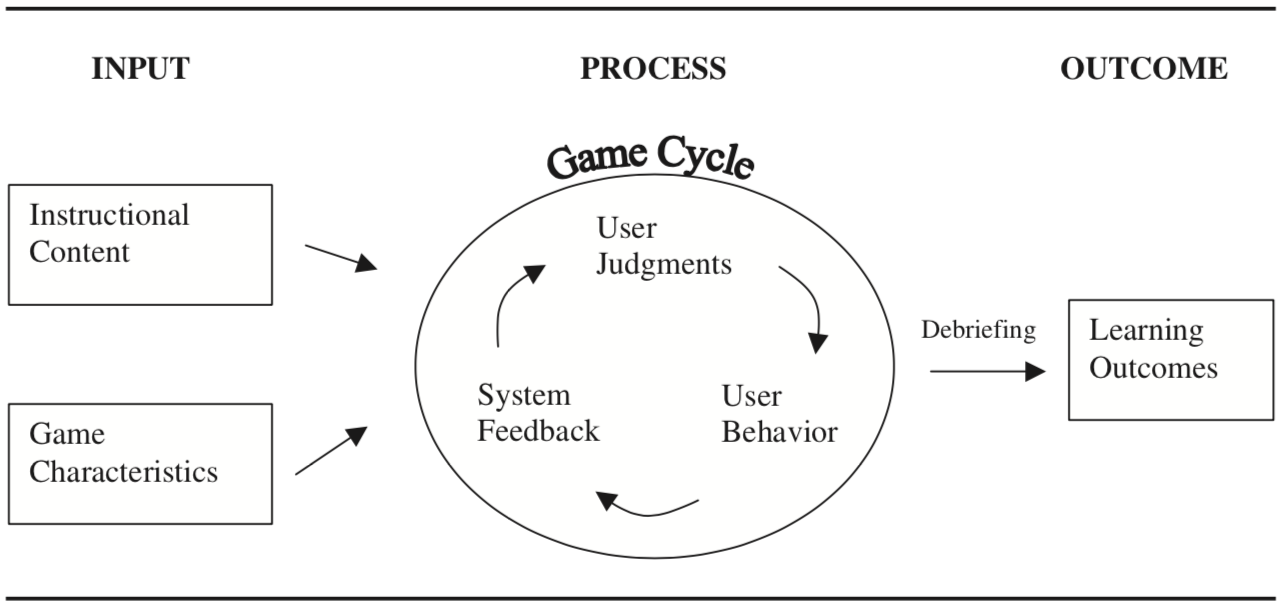
\includegraphics[width=1\textwidth]{Inputprocessoutcomegamemodel}
       \captionsetup{justification=centering}
\caption{Input-Process-Outcome Instructional Game Model  {\cite{Driskell2002}}}
\label{fig:Input_process_outcome_game_model}
\end{figure}

\subsection{Frameworks}

To be written.

EFM: A Model for Educational Game Design

\subsection{Game Design Elements}

(CHANGE IT UP) \citeauthor{Barnes2007} ran a project that made University Students create games that would teach basic programming. They carried out evaluations to test participant learning from the game, and made some interesting observations as follows: Clear instructions and game goals must be provided and accessible throughout the game, Learning goals must be clearly tied to in-game feedback that motivates the player (through, e.g. experience points, health), and penalizes guessing, Humor can be a motivation for in-game interaction \cite{Barnes2007}.

\subsubsection{Genre}

To be written.

\section{Resources for Teaching Programming}

To be written.

\afterpage{\blankpage}

\chapter{Requirements Specification}
\afterpage{\blankpage}

\chapter{Design}
\afterpage{\blankpage}

\chapter{Implementation}
\afterpage{\blankpage}

\chapter{Analysis and Testing}
\afterpage{\blankpage}

\chapter{Results}
\afterpage{\blankpage}

\chapter{Conclusions}
\afterpage{\blankpage}

\chapter{Future Work}
\afterpage{\blankpage}


\bibliography{litreview}
\bibliographystyle{plain}
\addcontentsline{toc}{chapter}{Bibliography}


\appendix
\addtocontents{toc}{\protect\setcounter{tocdepth}{-1}}
\addtocontents{toc}{\protect\setcounter{tocdepth}{0}}
\appendixpage

\renewcommand\chaptername{Appendix}
%\chapter{Technical Specification and GA of the Skyseeker}\label{app:techspec}

\newpage
\chapter{Uncertainty Analysis} \label{app:errors}

\chapter{Screenshots} \label{app:screenshots}

\chapter{Ethics Checklist} \label{app:ethicschecklist}

\end{document}  